\documentclass[twoside]{book}

% Packages required by doxygen
\usepackage{fixltx2e}
\usepackage{calc}
\usepackage{doxygen}
\usepackage[export]{adjustbox} % also loads graphicx
\usepackage{graphicx}
\usepackage[utf8]{inputenc}
\usepackage{makeidx}
\usepackage{multicol}
\usepackage{multirow}
\PassOptionsToPackage{warn}{textcomp}
\usepackage{textcomp}
\usepackage[nointegrals]{wasysym}
\usepackage[table]{xcolor}

% Font selection
\usepackage[T1]{fontenc}
\usepackage[scaled=.90]{helvet}
\usepackage{courier}
\usepackage{amssymb}
\usepackage{sectsty}
\renewcommand{\familydefault}{\sfdefault}
\allsectionsfont{%
  \fontseries{bc}\selectfont%
  \color{darkgray}%
}
\renewcommand{\DoxyLabelFont}{%
  \fontseries{bc}\selectfont%
  \color{darkgray}%
}
\newcommand{\+}{\discretionary{\mbox{\scriptsize$\hookleftarrow$}}{}{}}

% Page & text layout
\usepackage{geometry}
\geometry{%
  a4paper,%
  top=2.5cm,%
  bottom=2.5cm,%
  left=2.5cm,%
  right=2.5cm%
}
\tolerance=750
\hfuzz=15pt
\hbadness=750
\setlength{\emergencystretch}{15pt}
\setlength{\parindent}{0cm}
\setlength{\parskip}{3ex plus 2ex minus 2ex}
\makeatletter
\renewcommand{\paragraph}{%
  \@startsection{paragraph}{4}{0ex}{-1.0ex}{1.0ex}{%
    \normalfont\normalsize\bfseries\SS@parafont%
  }%
}
\renewcommand{\subparagraph}{%
  \@startsection{subparagraph}{5}{0ex}{-1.0ex}{1.0ex}{%
    \normalfont\normalsize\bfseries\SS@subparafont%
  }%
}
\makeatother

% Headers & footers
\usepackage{fancyhdr}
\pagestyle{fancyplain}
\fancyhead[LE]{\fancyplain{}{\bfseries\thepage}}
\fancyhead[CE]{\fancyplain{}{}}
\fancyhead[RE]{\fancyplain{}{\bfseries\leftmark}}
\fancyhead[LO]{\fancyplain{}{\bfseries\rightmark}}
\fancyhead[CO]{\fancyplain{}{}}
\fancyhead[RO]{\fancyplain{}{\bfseries\thepage}}
\fancyfoot[LE]{\fancyplain{}{}}
\fancyfoot[CE]{\fancyplain{}{}}
\fancyfoot[RE]{\fancyplain{}{\bfseries\scriptsize Generated by Doxygen }}
\fancyfoot[LO]{\fancyplain{}{\bfseries\scriptsize Generated by Doxygen }}
\fancyfoot[CO]{\fancyplain{}{}}
\fancyfoot[RO]{\fancyplain{}{}}
\renewcommand{\footrulewidth}{0.4pt}
\renewcommand{\chaptermark}[1]{%
  \markboth{#1}{}%
}
\renewcommand{\sectionmark}[1]{%
  \markright{\thesection\ #1}%
}

% Indices & bibliography
\usepackage{natbib}
\usepackage[titles]{tocloft}
\setcounter{tocdepth}{3}
\setcounter{secnumdepth}{5}
\makeindex

% Hyperlinks (required, but should be loaded last)
\usepackage{ifpdf}
\ifpdf
  \usepackage[pdftex,pagebackref=true]{hyperref}
\else
  \usepackage[ps2pdf,pagebackref=true]{hyperref}
\fi
\hypersetup{%
  colorlinks=true,%
  linkcolor=blue,%
  citecolor=blue,%
  unicode%
}

% Custom commands
\newcommand{\clearemptydoublepage}{%
  \newpage{\pagestyle{empty}\cleardoublepage}%
}

\usepackage{caption}
\captionsetup{labelsep=space,justification=centering,font={bf},singlelinecheck=off,skip=4pt,position=top}

%===== C O N T E N T S =====

\begin{document}

% Titlepage & ToC
\hypersetup{pageanchor=false,
             bookmarksnumbered=true,
             pdfencoding=unicode
            }
\pagenumbering{alph}
\begin{titlepage}
\vspace*{7cm}
\begin{center}%
{\Large Editor G\+UI Table }\\
\vspace*{1cm}
{\large Generated by Doxygen 1.8.14}\\
\end{center}
\end{titlepage}
\clearemptydoublepage
\pagenumbering{roman}
\tableofcontents
\clearemptydoublepage
\pagenumbering{arabic}
\hypersetup{pageanchor=true}

%--- Begin generated contents ---
\chapter{Namespace Index}
\section{Namespace List}
Here is a list of all documented namespaces with brief descriptions\+:\begin{DoxyCompactList}
\item\contentsline{section}{\mbox{\hyperlink{namespace_editor_g_u_i_table}{Editor\+G\+U\+I\+Table}} }{\pageref{namespace_editor_g_u_i_table}}{}
\end{DoxyCompactList}

\chapter{Hierarchical Index}
\section{Class Hierarchy}
This inheritance list is sorted roughly, but not completely, alphabetically\+:\begin{DoxyCompactList}
\item \contentsline{section}{G\+U\+I\+Extensions.\+G\+U\+I\+Table\+State}{\pageref{class_g_u_i_extensions_1_1_g_u_i_table_state}}{}
\item I\+Comparable\begin{DoxyCompactList}
\item \contentsline{section}{G\+U\+I\+Extensions.\+Table\+Entry}{\pageref{class_g_u_i_extensions_1_1_table_entry}}{}
\begin{DoxyCompactList}
\item \contentsline{section}{G\+U\+I\+Extensions.\+Action\+Entry}{\pageref{class_g_u_i_extensions_1_1_action_entry}}{}
\item \contentsline{section}{G\+U\+I\+Extensions.\+Label\+Entry}{\pageref{class_g_u_i_extensions_1_1_label_entry}}{}
\item \contentsline{section}{G\+U\+I\+Extensions.\+Property\+Entry}{\pageref{class_g_u_i_extensions_1_1_property_entry}}{}
\end{DoxyCompactList}
\end{DoxyCompactList}
\item \contentsline{section}{G\+U\+I\+Extensions.\+Table\+Column}{\pageref{class_g_u_i_extensions_1_1_table_column}}{}
\begin{DoxyCompactList}
\item \contentsline{section}{G\+U\+I\+Extensions.\+Property\+Column}{\pageref{class_g_u_i_extensions_1_1_property_column}}{}
\begin{DoxyCompactList}
\item \contentsline{section}{G\+U\+I\+Extensions.\+Selector\+Column}{\pageref{class_g_u_i_extensions_1_1_selector_column}}{}
\end{DoxyCompactList}
\end{DoxyCompactList}
\end{DoxyCompactList}

\chapter{Class Index}
\section{Class List}
Here are the classes, structs, unions and interfaces with brief descriptions\+:\begin{DoxyCompactList}
\item\contentsline{section}{\mbox{\hyperlink{class_editor_g_u_i_table_1_1_action_entry}{Editor\+G\+U\+I\+Table.\+Action\+Entry}} \\*This entry class draws a button which, when clicked, will trigger the action given in the constructor. }{\pageref{class_editor_g_u_i_table_1_1_action_entry}}{}
\item\contentsline{section}{\mbox{\hyperlink{class_editor_g_u_i_table_1_1_g_u_i_table_entry}{Editor\+G\+U\+I\+Table.\+G\+U\+I\+Table\+Entry}} }{\pageref{class_editor_g_u_i_table_1_1_g_u_i_table_entry}}{}
\item\contentsline{section}{\mbox{\hyperlink{class_editor_g_u_i_table_1_1_g_u_i_table_option}{Editor\+G\+U\+I\+Table.\+G\+U\+I\+Table\+Option}} }{\pageref{class_editor_g_u_i_table_1_1_g_u_i_table_option}}{}
\item\contentsline{section}{\mbox{\hyperlink{class_editor_g_u_i_table_1_1_g_u_i_table_state}{Editor\+G\+U\+I\+Table.\+G\+U\+I\+Table\+State}} \\*The current state of the G\+U\+I\+Table. This has to be used the same way state parameters are used in Unity G\+UI functions, like the scroll position in Begin\+Scroll\+View. It has to be passed from one G\+UI frame to another by keeping a reference in your calling code. }{\pageref{class_editor_g_u_i_table_1_1_g_u_i_table_state}}{}
\item\contentsline{section}{\mbox{\hyperlink{class_editor_g_u_i_table_1_1_label_entry}{Editor\+G\+U\+I\+Table.\+Label\+Entry}} \\*This entry class draws a string as a label. This is useful for properties you want to display in the table as read only, as the default Property\+Field used in \mbox{\hyperlink{class_editor_g_u_i_table_1_1_property_entry}{Property\+Entry}} uses editable fields. }{\pageref{class_editor_g_u_i_table_1_1_label_entry}}{}
\item\contentsline{section}{\mbox{\hyperlink{class_editor_g_u_i_table_1_1_property_column}{Editor\+G\+U\+I\+Table.\+Property\+Column}} \\*Internal Use Only. This class adds a property to a column. This will be used to automatically draw the entries for this column in some versions of G\+U\+I\+Table.\+Draw\+Table }{\pageref{class_editor_g_u_i_table_1_1_property_column}}{}
\item\contentsline{section}{\mbox{\hyperlink{class_editor_g_u_i_table_1_1_property_entry}{Editor\+G\+U\+I\+Table.\+Property\+Entry}} \\*This entry class just uses Editor\+G\+U\+I\+Layout.\+Property\+Field to draw a given property. This is the basic way to use G\+U\+I\+Table. It will draw the properties the same way Unity would by default. }{\pageref{class_editor_g_u_i_table_1_1_property_entry}}{}
\item\contentsline{section}{\mbox{\hyperlink{class_editor_g_u_i_table_1_1_selector_column}{Editor\+G\+U\+I\+Table.\+Selector\+Column}} \\*This class adds a property and a selector to a column. This will be used to automatically draw the entries for this column in some versions of G\+U\+I\+Table.\+Draw\+Table }{\pageref{class_editor_g_u_i_table_1_1_selector_column}}{}
\item\contentsline{section}{\mbox{\hyperlink{class_editor_g_u_i_table_1_1_table_column}{Editor\+G\+U\+I\+Table.\+Table\+Column}} \\*Base class for all table columns. It only takes a title and a width in the constructor, but other settings are available to customize the column. }{\pageref{class_editor_g_u_i_table_1_1_table_column}}{}
\item\contentsline{section}{\mbox{\hyperlink{class_table_column_entry}{Table\+Column\+Entry}} }{\pageref{class_table_column_entry}}{}
\item\contentsline{section}{\mbox{\hyperlink{class_table_column_option}{Table\+Column\+Option}} }{\pageref{class_table_column_option}}{}
\item\contentsline{section}{\mbox{\hyperlink{class_table_drawer}{Table\+Drawer}} \\*Drawer for the Table Attribute. See the Table\+Attribute class documentation for the limitations of this attribute. }{\pageref{class_table_drawer}}{}
\item\contentsline{section}{\mbox{\hyperlink{class_editor_g_u_i_table_1_1_table_entry}{Editor\+G\+U\+I\+Table.\+Table\+Entry}} \\*Base class for all table entries. Draw\+Entry needs to be overriden to draw the entry for the cell. Use this to customize the table however needed. Compare\+To can be overriden to customize the sorting. comparing\+Value is used as a fallback for sorting any types of entries, even different types. }{\pageref{class_editor_g_u_i_table_1_1_table_entry}}{}
\end{DoxyCompactList}

\chapter{Namespace Documentation}
\hypertarget{namespace_g_u_i_extensions}{}\section{G\+U\+I\+Extensions Namespace Reference}
\label{namespace_g_u_i_extensions}\index{G\+U\+I\+Extensions@{G\+U\+I\+Extensions}}
\subsection*{Classes}
\begin{DoxyCompactItemize}
\item 
class \mbox{\hyperlink{class_g_u_i_extensions_1_1_action_entry}{Action\+Entry}}
\begin{DoxyCompactList}\small\item\em This entry class draws a button which, when clicked, will trigger the action given in the constructor. \end{DoxyCompactList}\item 
class {\bfseries G\+U\+I\+Table}
\item 
class \mbox{\hyperlink{class_g_u_i_extensions_1_1_g_u_i_table_state}{G\+U\+I\+Table\+State}}
\begin{DoxyCompactList}\small\item\em The current state of the G\+U\+I\+Table. This has to be used the same way state parameters are used in Unity G\+UI functions, like the scroll position in Begin\+Scroll\+View. It has to be passed from one G\+UI frame to another by keeping a reference in your calling code. \end{DoxyCompactList}\item 
class \mbox{\hyperlink{class_g_u_i_extensions_1_1_label_entry}{Label\+Entry}}
\begin{DoxyCompactList}\small\item\em This entry class draws a string as a label. This is useful for properties you want to display in the table as read only, as the default Property\+Field used in \mbox{\hyperlink{class_g_u_i_extensions_1_1_property_entry}{Property\+Entry}} uses editable fields. \end{DoxyCompactList}\item 
class \mbox{\hyperlink{class_g_u_i_extensions_1_1_property_column}{Property\+Column}}
\begin{DoxyCompactList}\small\item\em Internal Use Only. This class adds a property to a column. This will be used to automatically draw the entries for this column in some versions of G\+U\+I\+Table.\+Draw\+Table \end{DoxyCompactList}\item 
class \mbox{\hyperlink{class_g_u_i_extensions_1_1_property_entry}{Property\+Entry}}
\begin{DoxyCompactList}\small\item\em This entry class just uses Editor\+G\+U\+I\+Layout.\+Property\+Field to draw a given property. This is the basic way to use G\+U\+I\+Table. It will draw the properties the same way Unity would by default. \end{DoxyCompactList}\item 
class \mbox{\hyperlink{class_g_u_i_extensions_1_1_selector_column}{Selector\+Column}}
\begin{DoxyCompactList}\small\item\em This class adds a property and a selector to a column. This will be used to automatically draw the entries for this column in some versions of G\+U\+I\+Table.\+Draw\+Table \end{DoxyCompactList}\item 
class \mbox{\hyperlink{class_g_u_i_extensions_1_1_table_column}{Table\+Column}}
\begin{DoxyCompactList}\small\item\em Base class for all table columns. It only takes a title and a width in the constructor, but other settings are available to customize the column. \end{DoxyCompactList}\item 
class \mbox{\hyperlink{class_g_u_i_extensions_1_1_table_entry}{Table\+Entry}}
\begin{DoxyCompactList}\small\item\em Base class for all table entries. Draw\+Entry needs to be overriden to draw the entry for the cell. Use this to customize the table however needed. Compare\+To can be overriden to customize the sorting. comparing\+Value is used as a fallback for sorting any types of entries, even different types. \end{DoxyCompactList}\end{DoxyCompactItemize}

\chapter{Class Documentation}
\hypertarget{class_g_u_i_extensions_1_1_action_entry}{}\section{G\+U\+I\+Extensions.\+Action\+Entry Class Reference}
\label{class_g_u_i_extensions_1_1_action_entry}\index{G\+U\+I\+Extensions.\+Action\+Entry@{G\+U\+I\+Extensions.\+Action\+Entry}}


This entry class draws a button which, when clicked, will trigger the action given in the constructor.  


Inheritance diagram for G\+U\+I\+Extensions.\+Action\+Entry\+:\begin{figure}[H]
\begin{center}
\leavevmode
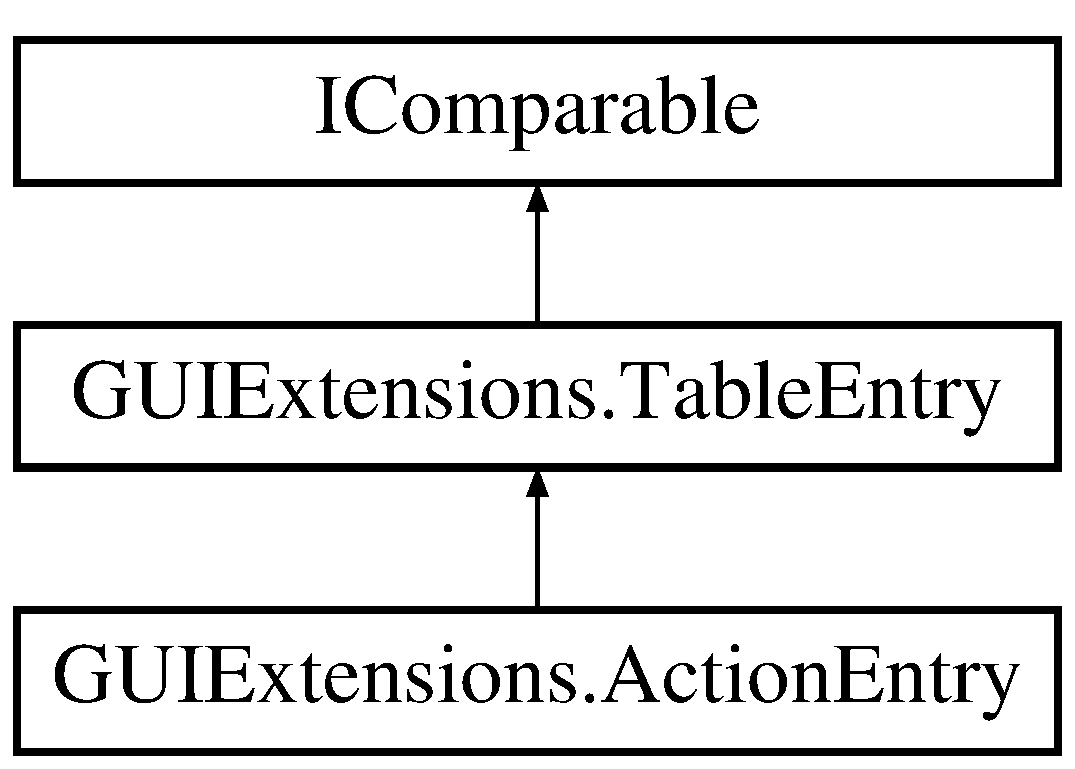
\includegraphics[height=3.000000cm]{class_g_u_i_extensions_1_1_action_entry}
\end{center}
\end{figure}
\subsection*{Public Member Functions}
\begin{DoxyCompactItemize}
\item 
\mbox{\Hypertarget{class_g_u_i_extensions_1_1_action_entry_a5718276960f5d27a0562e9327df64bbc}\label{class_g_u_i_extensions_1_1_action_entry_a5718276960f5d27a0562e9327df64bbc}} 
override void {\bfseries Draw\+Entry} (float width, float height)
\item 
\mbox{\Hypertarget{class_g_u_i_extensions_1_1_action_entry_adbb4bee6f9a29fa11978179fb6d24ff8}\label{class_g_u_i_extensions_1_1_action_entry_adbb4bee6f9a29fa11978179fb6d24ff8}} 
{\bfseries Action\+Entry} (string name, System.\+Action action)
\end{DoxyCompactItemize}
\subsection*{Properties}
\begin{DoxyCompactItemize}
\item 
\mbox{\Hypertarget{class_g_u_i_extensions_1_1_action_entry_ad2776be247baefb5c1ec443bd1244cfd}\label{class_g_u_i_extensions_1_1_action_entry_ad2776be247baefb5c1ec443bd1244cfd}} 
override string {\bfseries comparing\+Value}\hspace{0.3cm}{\ttfamily  \mbox{[}get\mbox{]}}
\end{DoxyCompactItemize}


\subsection{Detailed Description}
This entry class draws a button which, when clicked, will trigger the action given in the constructor. 



The documentation for this class was generated from the following file\+:\begin{DoxyCompactItemize}
\item 
/\+Users/jquentin/\+Documents/\+Projects/\+Editor\+G\+U\+I\+Table/\+Assets/\+G\+U\+I\+Table/\+Editor/\+Entries/Action\+Entry.\+cs\end{DoxyCompactItemize}

\hypertarget{class_g_u_i_extensions_1_1_g_u_i_table_state}{}\section{G\+U\+I\+Extensions.\+G\+U\+I\+Table\+State Class Reference}
\label{class_g_u_i_extensions_1_1_g_u_i_table_state}\index{G\+U\+I\+Extensions.\+G\+U\+I\+Table\+State@{G\+U\+I\+Extensions.\+G\+U\+I\+Table\+State}}


The current state of the G\+U\+I\+Table. This has to be used the same way state parameters are used in Unity G\+UI functions, like the scroll position in Begin\+Scroll\+View. It has to be passed from one G\+UI frame to another by keeping a reference in your calling code.  


\subsection*{Public Member Functions}
\begin{DoxyCompactItemize}
\item 
\mbox{\hyperlink{class_g_u_i_extensions_1_1_g_u_i_table_state_aa1c174fc584bf84ed57022fc04171298}{G\+U\+I\+Table\+State}} (string prefs\+Key)
\begin{DoxyCompactList}\small\item\em Initializes a \mbox{\hyperlink{class_g_u_i_extensions_1_1_g_u_i_table_state}{G\+U\+I\+Extensions.\+G\+U\+I\+Table\+State}} with a key to save it in Editor\+Prefs. This constructor can\textquotesingle{}t be used in Scriptable\+Object\textquotesingle{}s constructor or in the property\textquotesingle{}s declaration, because it uses the Editor\+Prefs. Use it in On\+Enable or Awake instead. \end{DoxyCompactList}\item 
\mbox{\Hypertarget{class_g_u_i_extensions_1_1_g_u_i_table_state_a2cabd40983f3ded2a1b8aaf2ffd6ecf5}\label{class_g_u_i_extensions_1_1_g_u_i_table_state_a2cabd40983f3ded2a1b8aaf2ffd6ecf5}} 
void {\bfseries Save} ()
\end{DoxyCompactItemize}
\subsection*{Static Public Member Functions}
\begin{DoxyCompactItemize}
\item 
\mbox{\Hypertarget{class_g_u_i_extensions_1_1_g_u_i_table_state_a15b8622c85e889c4ae225537684a9970}\label{class_g_u_i_extensions_1_1_g_u_i_table_state_a15b8622c85e889c4ae225537684a9970}} 
static \mbox{\hyperlink{class_g_u_i_extensions_1_1_g_u_i_table_state}{G\+U\+I\+Table\+State}} {\bfseries Load} (string prefs\+Key)
\end{DoxyCompactItemize}
\subsection*{Public Attributes}
\begin{DoxyCompactItemize}
\item 
\mbox{\Hypertarget{class_g_u_i_extensions_1_1_g_u_i_table_state_a8f3a30d048d0f19c1cb11451be849c24}\label{class_g_u_i_extensions_1_1_g_u_i_table_state_a8f3a30d048d0f19c1cb11451be849c24}} 
Vector2 {\bfseries scroll\+Pos}
\item 
\mbox{\Hypertarget{class_g_u_i_extensions_1_1_g_u_i_table_state_a28f1555aaef55d4ce9ea3b90d35c780c}\label{class_g_u_i_extensions_1_1_g_u_i_table_state_a28f1555aaef55d4ce9ea3b90d35c780c}} 
Vector2 {\bfseries scroll\+Pos\+Horiz}
\item 
\mbox{\Hypertarget{class_g_u_i_extensions_1_1_g_u_i_table_state_a8e062485d693d9d8204a8d868221f6a9}\label{class_g_u_i_extensions_1_1_g_u_i_table_state_a8e062485d693d9d8204a8d868221f6a9}} 
int {\bfseries sort\+By\+Column\+Index} = -\/1
\item 
\mbox{\Hypertarget{class_g_u_i_extensions_1_1_g_u_i_table_state_aa0dd82f8c71eac659a8774d61fd4fbfd}\label{class_g_u_i_extensions_1_1_g_u_i_table_state_aa0dd82f8c71eac659a8774d61fd4fbfd}} 
bool {\bfseries sort\+Increasing}
\item 
\mbox{\Hypertarget{class_g_u_i_extensions_1_1_g_u_i_table_state_a07122241ee02f8d8c31f0908d67f1bd5}\label{class_g_u_i_extensions_1_1_g_u_i_table_state_a07122241ee02f8d8c31f0908d67f1bd5}} 
List$<$ float $>$ {\bfseries column\+Sizes} = new List$<$float$>$ ()
\item 
\mbox{\Hypertarget{class_g_u_i_extensions_1_1_g_u_i_table_state_a2612ab7ea11c0a56c961dc4f93470e10}\label{class_g_u_i_extensions_1_1_g_u_i_table_state_a2612ab7ea11c0a56c961dc4f93470e10}} 
List$<$ bool $>$ {\bfseries column\+Visible} = new List$<$bool$>$ ()
\end{DoxyCompactItemize}


\subsection{Detailed Description}
The current state of the G\+U\+I\+Table. This has to be used the same way state parameters are used in Unity G\+UI functions, like the scroll position in Begin\+Scroll\+View. It has to be passed from one G\+UI frame to another by keeping a reference in your calling code. 


\begin{DoxyCode}
GUITableState tableState;
\textcolor{keywordtype}{void} OnGUI ()
\{
    tableState = GUITable.DrawTable(collectionProperty, tableState);
\}
\end{DoxyCode}
 

\subsection{Constructor \& Destructor Documentation}
\mbox{\Hypertarget{class_g_u_i_extensions_1_1_g_u_i_table_state_aa1c174fc584bf84ed57022fc04171298}\label{class_g_u_i_extensions_1_1_g_u_i_table_state_aa1c174fc584bf84ed57022fc04171298}} 
\index{G\+U\+I\+Extensions\+::\+G\+U\+I\+Table\+State@{G\+U\+I\+Extensions\+::\+G\+U\+I\+Table\+State}!G\+U\+I\+Table\+State@{G\+U\+I\+Table\+State}}
\index{G\+U\+I\+Table\+State@{G\+U\+I\+Table\+State}!G\+U\+I\+Extensions\+::\+G\+U\+I\+Table\+State@{G\+U\+I\+Extensions\+::\+G\+U\+I\+Table\+State}}
\subsubsection{\texorpdfstring{G\+U\+I\+Table\+State()}{GUITableState()}}
{\footnotesize\ttfamily G\+U\+I\+Extensions.\+G\+U\+I\+Table\+State.\+G\+U\+I\+Table\+State (\begin{DoxyParamCaption}\item[{string}]{prefs\+Key }\end{DoxyParamCaption})}



Initializes a \mbox{\hyperlink{class_g_u_i_extensions_1_1_g_u_i_table_state}{G\+U\+I\+Extensions.\+G\+U\+I\+Table\+State}} with a key to save it in Editor\+Prefs. This constructor can\textquotesingle{}t be used in Scriptable\+Object\textquotesingle{}s constructor or in the property\textquotesingle{}s declaration, because it uses the Editor\+Prefs. Use it in On\+Enable or Awake instead. 


\begin{DoxyParams}{Parameters}
{\em prefs\+Key} & Prefs key.\\
\hline
\end{DoxyParams}


The documentation for this class was generated from the following file\+:\begin{DoxyCompactItemize}
\item 
/\+Users/jquentin/\+Documents/\+Projects/\+Editor\+G\+U\+I\+Table/\+Assets/\+G\+U\+I\+Table/\+Editor/G\+U\+I\+Table\+State.\+cs\end{DoxyCompactItemize}

\hypertarget{class_g_u_i_extensions_1_1_label_entry}{}\section{G\+U\+I\+Extensions.\+Label\+Entry Class Reference}
\label{class_g_u_i_extensions_1_1_label_entry}\index{G\+U\+I\+Extensions.\+Label\+Entry@{G\+U\+I\+Extensions.\+Label\+Entry}}


This entry class draws a string as a label. This is useful for properties you want to display in the table as read only, as the default Property\+Field used in \mbox{\hyperlink{class_g_u_i_extensions_1_1_property_entry}{Property\+Entry}} uses editable fields.  


Inheritance diagram for G\+U\+I\+Extensions.\+Label\+Entry\+:\begin{figure}[H]
\begin{center}
\leavevmode
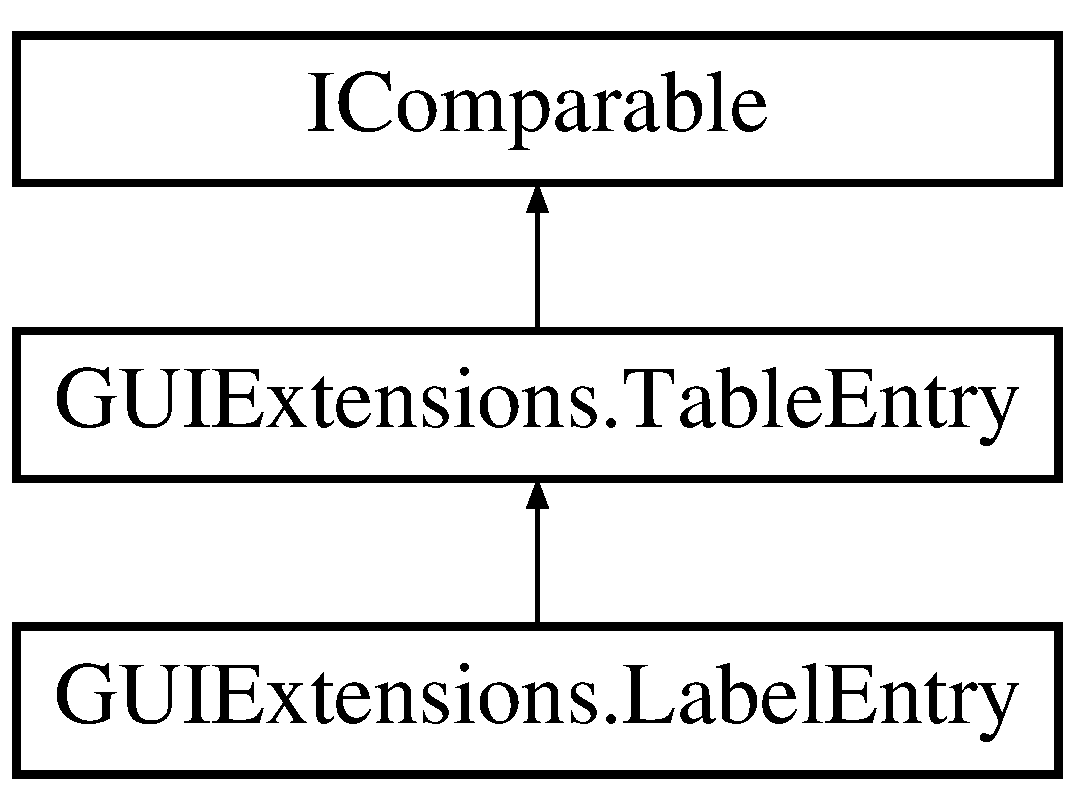
\includegraphics[height=3.000000cm]{class_g_u_i_extensions_1_1_label_entry}
\end{center}
\end{figure}
\subsection*{Public Member Functions}
\begin{DoxyCompactItemize}
\item 
\mbox{\Hypertarget{class_g_u_i_extensions_1_1_label_entry_acd1df46f271a40e97c396c6099c0e9f5}\label{class_g_u_i_extensions_1_1_label_entry_acd1df46f271a40e97c396c6099c0e9f5}} 
override void {\bfseries Draw\+Entry} (float width, float height)
\item 
\mbox{\Hypertarget{class_g_u_i_extensions_1_1_label_entry_a40cd1ac009a43e0a6286e6feca39c60a}\label{class_g_u_i_extensions_1_1_label_entry_a40cd1ac009a43e0a6286e6feca39c60a}} 
{\bfseries Label\+Entry} (string value)
\end{DoxyCompactItemize}
\subsection*{Properties}
\begin{DoxyCompactItemize}
\item 
\mbox{\Hypertarget{class_g_u_i_extensions_1_1_label_entry_ab0ee942386b9a1471250f468ec41acf6}\label{class_g_u_i_extensions_1_1_label_entry_ab0ee942386b9a1471250f468ec41acf6}} 
override string {\bfseries comparing\+Value}\hspace{0.3cm}{\ttfamily  \mbox{[}get\mbox{]}}
\end{DoxyCompactItemize}


\subsection{Detailed Description}
This entry class draws a string as a label. This is useful for properties you want to display in the table as read only, as the default Property\+Field used in \mbox{\hyperlink{class_g_u_i_extensions_1_1_property_entry}{Property\+Entry}} uses editable fields. 



The documentation for this class was generated from the following file\+:\begin{DoxyCompactItemize}
\item 
/\+Users/jquentin/\+Documents/\+Projects/\+Editor\+G\+U\+I\+Table/\+Assets/\+G\+U\+I\+Table/\+Editor/\+Entries/Label\+Entry.\+cs\end{DoxyCompactItemize}

\hypertarget{class_g_u_i_extensions_1_1_property_column}{}\section{G\+U\+I\+Extensions.\+Property\+Column Class Reference}
\label{class_g_u_i_extensions_1_1_property_column}\index{G\+U\+I\+Extensions.\+Property\+Column@{G\+U\+I\+Extensions.\+Property\+Column}}


Internal Use Only. This class adds a property to a column. This will be used to automatically draw the entries for this column in some versions of G\+U\+I\+Table.\+Draw\+Table  


Inheritance diagram for G\+U\+I\+Extensions.\+Property\+Column\+:\begin{figure}[H]
\begin{center}
\leavevmode
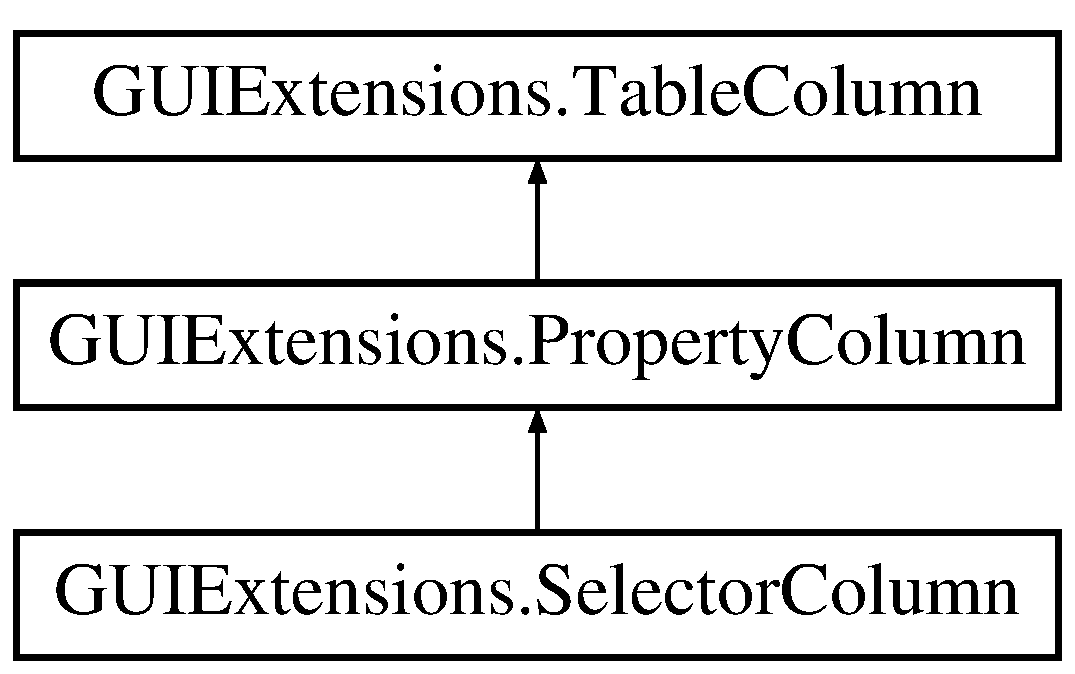
\includegraphics[height=3.000000cm]{class_g_u_i_extensions_1_1_property_column}
\end{center}
\end{figure}
\subsection*{Public Member Functions}
\begin{DoxyCompactItemize}
\item 
\mbox{\Hypertarget{class_g_u_i_extensions_1_1_property_column_a9e5b8655054132f351926de205a3f2aa}\label{class_g_u_i_extensions_1_1_property_column_a9e5b8655054132f351926de205a3f2aa}} 
{\bfseries Property\+Column} (string property\+Name, string name, float width)
\end{DoxyCompactItemize}
\subsection*{Public Attributes}
\begin{DoxyCompactItemize}
\item 
\mbox{\Hypertarget{class_g_u_i_extensions_1_1_property_column_afd70f617ed70ba8f14747115e5b957ec}\label{class_g_u_i_extensions_1_1_property_column_afd70f617ed70ba8f14747115e5b957ec}} 
string {\bfseries property\+Name}
\end{DoxyCompactItemize}
\subsection*{Additional Inherited Members}


\subsection{Detailed Description}
Internal Use Only. This class adds a property to a column. This will be used to automatically draw the entries for this column in some versions of G\+U\+I\+Table.\+Draw\+Table 



The documentation for this class was generated from the following file\+:\begin{DoxyCompactItemize}
\item 
/\+Users/jquentin/\+Documents/\+Projects/\+Editor\+G\+U\+I\+Table/\+Assets/\+G\+U\+I\+Table/\+Editor/\+Columns/Property\+Column.\+cs\end{DoxyCompactItemize}

\hypertarget{class_g_u_i_extensions_1_1_property_entry}{}\section{G\+U\+I\+Extensions.\+Property\+Entry Class Reference}
\label{class_g_u_i_extensions_1_1_property_entry}\index{G\+U\+I\+Extensions.\+Property\+Entry@{G\+U\+I\+Extensions.\+Property\+Entry}}


This entry class just uses Editor\+G\+U\+I\+Layout.\+Property\+Field to draw a given property. This is the basic way to use G\+U\+I\+Table. It will draw the properties the same way Unity would by default.  


Inheritance diagram for G\+U\+I\+Extensions.\+Property\+Entry\+:\begin{figure}[H]
\begin{center}
\leavevmode
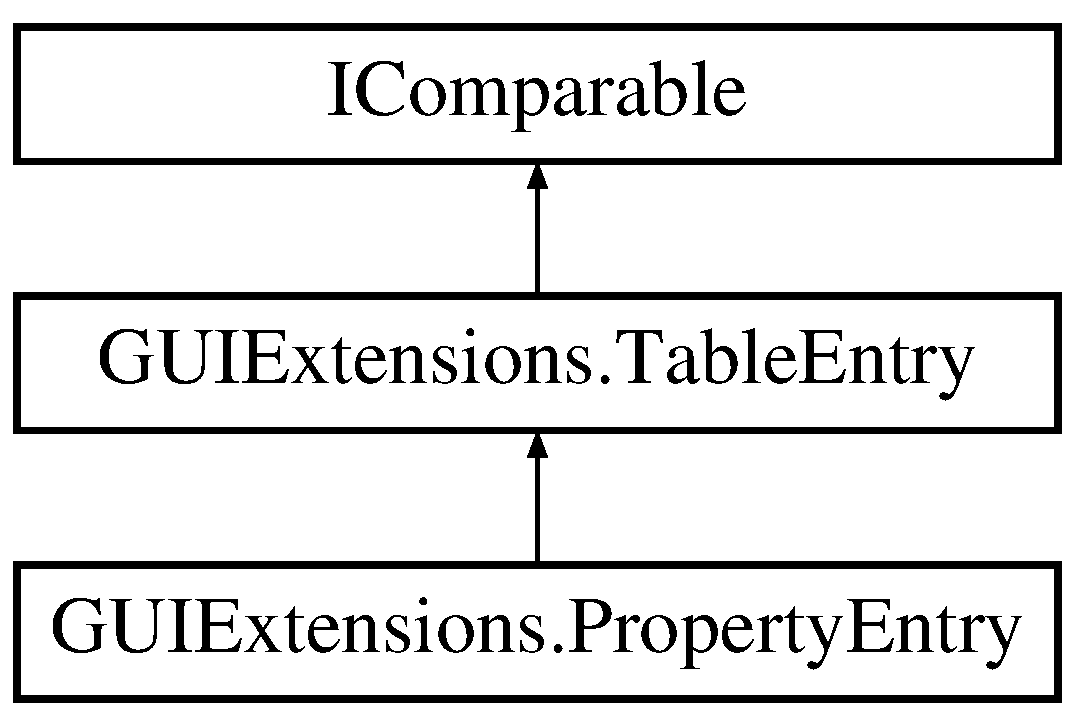
\includegraphics[height=3.000000cm]{class_g_u_i_extensions_1_1_property_entry}
\end{center}
\end{figure}
\subsection*{Public Member Functions}
\begin{DoxyCompactItemize}
\item 
\mbox{\Hypertarget{class_g_u_i_extensions_1_1_property_entry_a30717a2d99776193e1aaea13de2eb517}\label{class_g_u_i_extensions_1_1_property_entry_a30717a2d99776193e1aaea13de2eb517}} 
override void {\bfseries Draw\+Entry} (float width, float height)
\item 
\mbox{\Hypertarget{class_g_u_i_extensions_1_1_property_entry_a38fa06c9db5fb809e819b32e5f6364de}\label{class_g_u_i_extensions_1_1_property_entry_a38fa06c9db5fb809e819b32e5f6364de}} 
override int {\bfseries Compare\+To} (object other)
\item 
\mbox{\Hypertarget{class_g_u_i_extensions_1_1_property_entry_a10e29d4bb2e12a2f761c801999a732c2}\label{class_g_u_i_extensions_1_1_property_entry_a10e29d4bb2e12a2f761c801999a732c2}} 
{\bfseries Property\+Entry} (Serialized\+Object so, string property\+Name)
\end{DoxyCompactItemize}
\subsection*{Properties}
\begin{DoxyCompactItemize}
\item 
\mbox{\Hypertarget{class_g_u_i_extensions_1_1_property_entry_a40ce6bba52176b88be69536e4a0c4258}\label{class_g_u_i_extensions_1_1_property_entry_a40ce6bba52176b88be69536e4a0c4258}} 
override string {\bfseries comparing\+Value}\hspace{0.3cm}{\ttfamily  \mbox{[}get\mbox{]}}
\end{DoxyCompactItemize}


\subsection{Detailed Description}
This entry class just uses Editor\+G\+U\+I\+Layout.\+Property\+Field to draw a given property. This is the basic way to use G\+U\+I\+Table. It will draw the properties the same way Unity would by default. 



The documentation for this class was generated from the following file\+:\begin{DoxyCompactItemize}
\item 
/\+Users/jquentin/\+Documents/\+Projects/\+Editor\+G\+U\+I\+Table/\+Assets/\+G\+U\+I\+Table/\+Editor/\+Entries/Property\+Entry.\+cs\end{DoxyCompactItemize}

\hypertarget{class_g_u_i_extensions_1_1_selector_column}{}\section{G\+U\+I\+Extensions.\+Selector\+Column Class Reference}
\label{class_g_u_i_extensions_1_1_selector_column}\index{G\+U\+I\+Extensions.\+Selector\+Column@{G\+U\+I\+Extensions.\+Selector\+Column}}


This class adds a property and a selector to a column. This will be used to automatically draw the entries for this column in some versions of G\+U\+I\+Table.\+Draw\+Table  


Inheritance diagram for G\+U\+I\+Extensions.\+Selector\+Column\+:\begin{figure}[H]
\begin{center}
\leavevmode
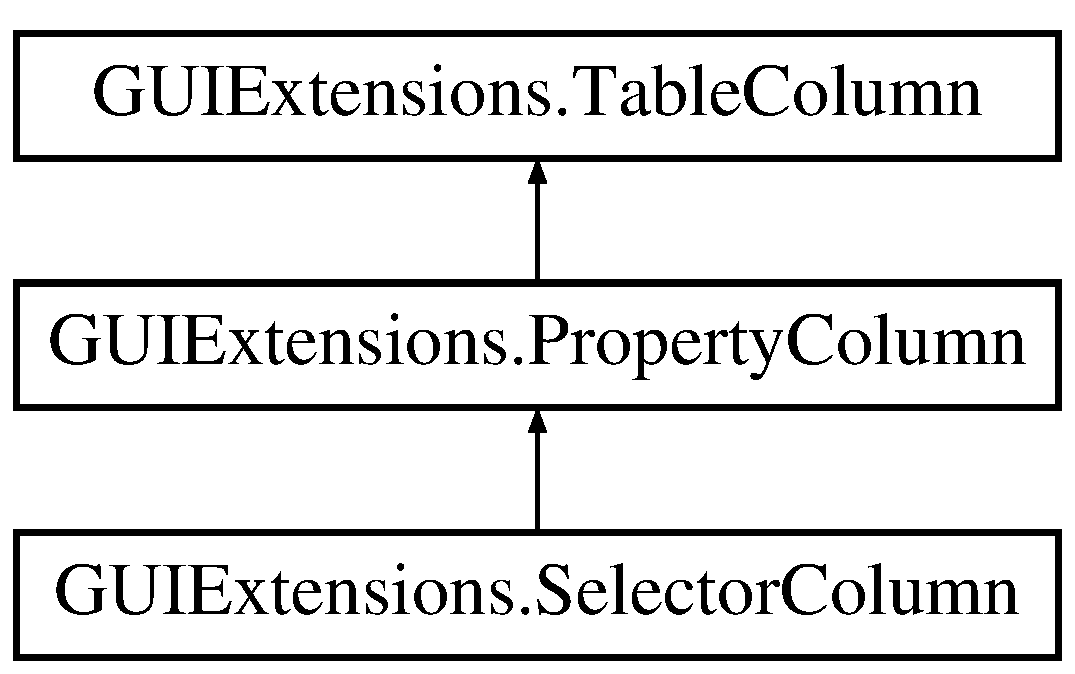
\includegraphics[height=3.000000cm]{class_g_u_i_extensions_1_1_selector_column}
\end{center}
\end{figure}
\subsection*{Public Member Functions}
\begin{DoxyCompactItemize}
\item 
\mbox{\Hypertarget{class_g_u_i_extensions_1_1_selector_column_aa1c9ebb87dc3d5043aef0ffa48765572}\label{class_g_u_i_extensions_1_1_selector_column_aa1c9ebb87dc3d5043aef0ffa48765572}} 
{\bfseries Selector\+Column} (Func$<$ Serialized\+Property, \mbox{\hyperlink{class_g_u_i_extensions_1_1_table_entry}{Table\+Entry}} $>$ selector, string property\+Name, string name, float width)
\end{DoxyCompactItemize}
\subsection*{Public Attributes}
\begin{DoxyCompactItemize}
\item 
\mbox{\Hypertarget{class_g_u_i_extensions_1_1_selector_column_a9b19236c8e6d155923d8b42485d7da4f}\label{class_g_u_i_extensions_1_1_selector_column_a9b19236c8e6d155923d8b42485d7da4f}} 
Func$<$ Serialized\+Property, \mbox{\hyperlink{class_g_u_i_extensions_1_1_table_entry}{Table\+Entry}} $>$ {\bfseries selector}
\end{DoxyCompactItemize}
\subsection*{Additional Inherited Members}


\subsection{Detailed Description}
This class adds a property and a selector to a column. This will be used to automatically draw the entries for this column in some versions of G\+U\+I\+Table.\+Draw\+Table 



The documentation for this class was generated from the following file\+:\begin{DoxyCompactItemize}
\item 
/\+Users/jquentin/\+Documents/\+Projects/\+Editor\+G\+U\+I\+Table/\+Assets/\+G\+U\+I\+Table/\+Editor/\+Columns/Selector\+Column.\+cs\end{DoxyCompactItemize}

\hypertarget{class_g_u_i_extensions_1_1_table_column}{}\section{G\+U\+I\+Extensions.\+Table\+Column Class Reference}
\label{class_g_u_i_extensions_1_1_table_column}\index{G\+U\+I\+Extensions.\+Table\+Column@{G\+U\+I\+Extensions.\+Table\+Column}}


Base class for all table columns. It only takes a title and a width in the constructor, but other settings are available to customize the column.  


Inheritance diagram for G\+U\+I\+Extensions.\+Table\+Column\+:\begin{figure}[H]
\begin{center}
\leavevmode
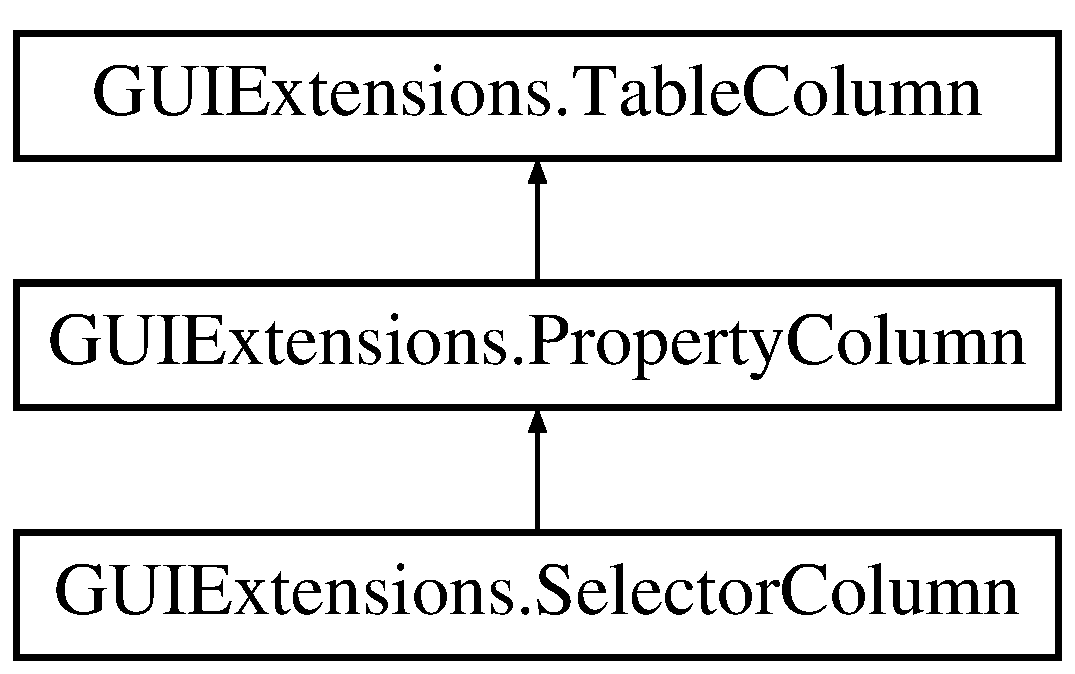
\includegraphics[height=3.000000cm]{class_g_u_i_extensions_1_1_table_column}
\end{center}
\end{figure}
\subsection*{Public Member Functions}
\begin{DoxyCompactItemize}
\item 
\mbox{\hyperlink{class_g_u_i_extensions_1_1_table_column_a27389bffc8435c64dbdc03c96d396383}{Table\+Column}} (string title, float width)
\begin{DoxyCompactList}\small\item\em Initializes a column with its title and width. Edit the other public properties for more settings. \end{DoxyCompactList}\end{DoxyCompactItemize}
\subsection*{Public Attributes}
\begin{DoxyCompactItemize}
\item 
bool \mbox{\hyperlink{class_g_u_i_extensions_1_1_table_column_a6c4958c3bcf3a93a78d575c9a41776fe}{enabled\+Entries}} = true
\begin{DoxyCompactList}\small\item\em Defines if the entries are enabled (interactable) or disabled (grayed out). Default\+: true. \end{DoxyCompactList}\item 
bool \mbox{\hyperlink{class_g_u_i_extensions_1_1_table_column_ad46a3aeba25051869bcad488eaa6f9dc}{is\+Sortable}} = true
\begin{DoxyCompactList}\small\item\em Defines if the column is sortable. \end{DoxyCompactList}\item 
bool \mbox{\hyperlink{class_g_u_i_extensions_1_1_table_column_a9fe6044251cdd55a22469a638ead7d7f}{enabled\+Title}} = true
\begin{DoxyCompactList}\small\item\em Defines if the title is enabled (interactable) or disabled (grayed out). Default\+: true. \end{DoxyCompactList}\item 
bool \mbox{\hyperlink{class_g_u_i_extensions_1_1_table_column_ac09648f6d91b018cae5c80bcd7499630}{optional}} = false
\begin{DoxyCompactList}\small\item\em Defines if the column can be hidden by right-\/clicking the column titles bar. Default\+: false. \end{DoxyCompactList}\item 
bool \mbox{\hyperlink{class_g_u_i_extensions_1_1_table_column_af0cd04c373e963e227a4bfb4da234f77}{visible\+By\+Default}} = true
\begin{DoxyCompactList}\small\item\em Defines if the column is visible by default. If this is false, and optional is false too. The column can never be viewed. Default\+: true. \end{DoxyCompactList}\end{DoxyCompactItemize}
\subsection*{Properties}
\begin{DoxyCompactItemize}
\item 
\mbox{\Hypertarget{class_g_u_i_extensions_1_1_table_column_aaaec6ba370e158472aac5940a943b117}\label{class_g_u_i_extensions_1_1_table_column_aaaec6ba370e158472aac5940a943b117}} 
string {\bfseries title}\hspace{0.3cm}{\ttfamily  \mbox{[}get\mbox{]}}
\item 
\mbox{\Hypertarget{class_g_u_i_extensions_1_1_table_column_a07863be1efd646e6238399f2cccfd9f2}\label{class_g_u_i_extensions_1_1_table_column_a07863be1efd646e6238399f2cccfd9f2}} 
float {\bfseries width}\hspace{0.3cm}{\ttfamily  \mbox{[}get\mbox{]}}
\end{DoxyCompactItemize}


\subsection{Detailed Description}
Base class for all table columns. It only takes a title and a width in the constructor, but other settings are available to customize the column. 



\subsection{Constructor \& Destructor Documentation}
\mbox{\Hypertarget{class_g_u_i_extensions_1_1_table_column_a27389bffc8435c64dbdc03c96d396383}\label{class_g_u_i_extensions_1_1_table_column_a27389bffc8435c64dbdc03c96d396383}} 
\index{G\+U\+I\+Extensions\+::\+Table\+Column@{G\+U\+I\+Extensions\+::\+Table\+Column}!Table\+Column@{Table\+Column}}
\index{Table\+Column@{Table\+Column}!G\+U\+I\+Extensions\+::\+Table\+Column@{G\+U\+I\+Extensions\+::\+Table\+Column}}
\subsubsection{\texorpdfstring{Table\+Column()}{TableColumn()}}
{\footnotesize\ttfamily G\+U\+I\+Extensions.\+Table\+Column.\+Table\+Column (\begin{DoxyParamCaption}\item[{string}]{title,  }\item[{float}]{width }\end{DoxyParamCaption})}



Initializes a column with its title and width. Edit the other public properties for more settings. 


\begin{DoxyParams}{Parameters}
{\em title} & The column title.\\
\hline
{\em width} & The column width.\\
\hline
\end{DoxyParams}


\subsection{Member Data Documentation}
\mbox{\Hypertarget{class_g_u_i_extensions_1_1_table_column_a6c4958c3bcf3a93a78d575c9a41776fe}\label{class_g_u_i_extensions_1_1_table_column_a6c4958c3bcf3a93a78d575c9a41776fe}} 
\index{G\+U\+I\+Extensions\+::\+Table\+Column@{G\+U\+I\+Extensions\+::\+Table\+Column}!enabled\+Entries@{enabled\+Entries}}
\index{enabled\+Entries@{enabled\+Entries}!G\+U\+I\+Extensions\+::\+Table\+Column@{G\+U\+I\+Extensions\+::\+Table\+Column}}
\subsubsection{\texorpdfstring{enabled\+Entries}{enabledEntries}}
{\footnotesize\ttfamily bool G\+U\+I\+Extensions.\+Table\+Column.\+enabled\+Entries = true}



Defines if the entries are enabled (interactable) or disabled (grayed out). Default\+: true. 

\mbox{\Hypertarget{class_g_u_i_extensions_1_1_table_column_a9fe6044251cdd55a22469a638ead7d7f}\label{class_g_u_i_extensions_1_1_table_column_a9fe6044251cdd55a22469a638ead7d7f}} 
\index{G\+U\+I\+Extensions\+::\+Table\+Column@{G\+U\+I\+Extensions\+::\+Table\+Column}!enabled\+Title@{enabled\+Title}}
\index{enabled\+Title@{enabled\+Title}!G\+U\+I\+Extensions\+::\+Table\+Column@{G\+U\+I\+Extensions\+::\+Table\+Column}}
\subsubsection{\texorpdfstring{enabled\+Title}{enabledTitle}}
{\footnotesize\ttfamily bool G\+U\+I\+Extensions.\+Table\+Column.\+enabled\+Title = true}



Defines if the title is enabled (interactable) or disabled (grayed out). Default\+: true. 

\mbox{\Hypertarget{class_g_u_i_extensions_1_1_table_column_ad46a3aeba25051869bcad488eaa6f9dc}\label{class_g_u_i_extensions_1_1_table_column_ad46a3aeba25051869bcad488eaa6f9dc}} 
\index{G\+U\+I\+Extensions\+::\+Table\+Column@{G\+U\+I\+Extensions\+::\+Table\+Column}!is\+Sortable@{is\+Sortable}}
\index{is\+Sortable@{is\+Sortable}!G\+U\+I\+Extensions\+::\+Table\+Column@{G\+U\+I\+Extensions\+::\+Table\+Column}}
\subsubsection{\texorpdfstring{is\+Sortable}{isSortable}}
{\footnotesize\ttfamily bool G\+U\+I\+Extensions.\+Table\+Column.\+is\+Sortable = true}



Defines if the column is sortable. 

\mbox{\Hypertarget{class_g_u_i_extensions_1_1_table_column_ac09648f6d91b018cae5c80bcd7499630}\label{class_g_u_i_extensions_1_1_table_column_ac09648f6d91b018cae5c80bcd7499630}} 
\index{G\+U\+I\+Extensions\+::\+Table\+Column@{G\+U\+I\+Extensions\+::\+Table\+Column}!optional@{optional}}
\index{optional@{optional}!G\+U\+I\+Extensions\+::\+Table\+Column@{G\+U\+I\+Extensions\+::\+Table\+Column}}
\subsubsection{\texorpdfstring{optional}{optional}}
{\footnotesize\ttfamily bool G\+U\+I\+Extensions.\+Table\+Column.\+optional = false}



Defines if the column can be hidden by right-\/clicking the column titles bar. Default\+: false. 

\mbox{\Hypertarget{class_g_u_i_extensions_1_1_table_column_af0cd04c373e963e227a4bfb4da234f77}\label{class_g_u_i_extensions_1_1_table_column_af0cd04c373e963e227a4bfb4da234f77}} 
\index{G\+U\+I\+Extensions\+::\+Table\+Column@{G\+U\+I\+Extensions\+::\+Table\+Column}!visible\+By\+Default@{visible\+By\+Default}}
\index{visible\+By\+Default@{visible\+By\+Default}!G\+U\+I\+Extensions\+::\+Table\+Column@{G\+U\+I\+Extensions\+::\+Table\+Column}}
\subsubsection{\texorpdfstring{visible\+By\+Default}{visibleByDefault}}
{\footnotesize\ttfamily bool G\+U\+I\+Extensions.\+Table\+Column.\+visible\+By\+Default = true}



Defines if the column is visible by default. If this is false, and optional is false too. The column can never be viewed. Default\+: true. 



The documentation for this class was generated from the following file\+:\begin{DoxyCompactItemize}
\item 
/\+Users/jquentin/\+Documents/\+Projects/\+Editor\+G\+U\+I\+Table/\+Assets/\+G\+U\+I\+Table/\+Editor/\+Columns/Table\+Column.\+cs\end{DoxyCompactItemize}

\hypertarget{class_g_u_i_extensions_1_1_table_entry}{}\section{G\+U\+I\+Extensions.\+Table\+Entry Class Reference}
\label{class_g_u_i_extensions_1_1_table_entry}\index{G\+U\+I\+Extensions.\+Table\+Entry@{G\+U\+I\+Extensions.\+Table\+Entry}}


Base class for all table entries. Draw\+Entry needs to be overriden to draw the entry for the cell. Use this to customize the table however needed. Compare\+To can be overriden to customize the sorting. comparing\+Value is used as a fallback for sorting any types of entries, even different types.  


Inheritance diagram for G\+U\+I\+Extensions.\+Table\+Entry\+:\begin{figure}[H]
\begin{center}
\leavevmode
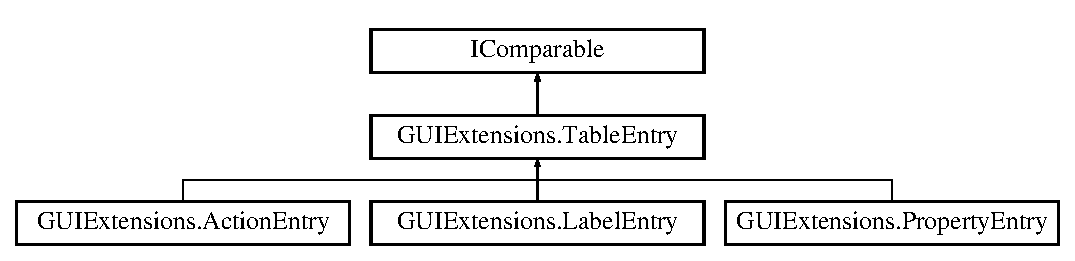
\includegraphics[height=3.000000cm]{class_g_u_i_extensions_1_1_table_entry}
\end{center}
\end{figure}
\subsection*{Public Member Functions}
\begin{DoxyCompactItemize}
\item 
\mbox{\Hypertarget{class_g_u_i_extensions_1_1_table_entry_a016546c12c86e693840a15b74a775bb0}\label{class_g_u_i_extensions_1_1_table_entry_a016546c12c86e693840a15b74a775bb0}} 
abstract void {\bfseries Draw\+Entry} (float width, float height)
\item 
\mbox{\Hypertarget{class_g_u_i_extensions_1_1_table_entry_a9d148f0b0dd7c1b08ce1d38378164798}\label{class_g_u_i_extensions_1_1_table_entry_a9d148f0b0dd7c1b08ce1d38378164798}} 
virtual int {\bfseries Compare\+To} (object other)
\end{DoxyCompactItemize}
\subsection*{Properties}
\begin{DoxyCompactItemize}
\item 
\mbox{\Hypertarget{class_g_u_i_extensions_1_1_table_entry_a75a4c1aab5335e83969f4e04f6fbb83c}\label{class_g_u_i_extensions_1_1_table_entry_a75a4c1aab5335e83969f4e04f6fbb83c}} 
abstract string {\bfseries comparing\+Value}\hspace{0.3cm}{\ttfamily  \mbox{[}get\mbox{]}}
\end{DoxyCompactItemize}


\subsection{Detailed Description}
Base class for all table entries. Draw\+Entry needs to be overriden to draw the entry for the cell. Use this to customize the table however needed. Compare\+To can be overriden to customize the sorting. comparing\+Value is used as a fallback for sorting any types of entries, even different types. 



The documentation for this class was generated from the following file\+:\begin{DoxyCompactItemize}
\item 
/\+Users/jquentin/\+Documents/\+Projects/\+Editor\+G\+U\+I\+Table/\+Assets/\+G\+U\+I\+Table/\+Editor/\+Entries/Table\+Entry.\+cs\end{DoxyCompactItemize}

%--- End generated contents ---

% Index
\backmatter
\newpage
\phantomsection
\clearemptydoublepage
\addcontentsline{toc}{chapter}{Index}
\printindex

\end{document}
